\section{Cadhier des charges}

\subsection{Objectif du circuit}

Le contrôleur I2C a pour rôle d'assurer le couplage du processeur avec son
environnement extérieur via une liaison série de type I2C (signaux SCL et SDA). Il
fonctionne en mode maître : il génère l'horloge SCL, les conditions START et STOP, émet
l'adresse de l'esclave, puis émet ou reçoit une suite d'octets selon la configuration
programmée par le processeur.
\\

\subsection{Fonctionnalités attendues}

Les fonctions de service du circuit sont :
\\

\begin{itemize}
    \item Le circuit peut être configuré par le processeur, la configuration porte sur :
    \begin{enumerate}
        \item la vitesse de transmission : 100 kbit/s (mode standard) ou 400 kbit/s (mode rapide),
        \item la génération d'une interruption en fin de transaction (avec ou sans),
        \item le sens du transfert : écriture (maître vers esclave) ou lecture (esclave vers maître),
        \item le nombre d'octets de données à transmettre ou à recevoir (de 1 à 8),
        \item l'adresse de l'esclave visé (7 bits).
    \end{enumerate}
    \item Le circuit peut émettre une trame I2C : START, adresse + bit R/W, octets de données avec acquittement, STOP.
    \item Le circuit peut recevoir une suite d'octets en provenance de l'esclave, acquitter chaque octet (ACK) et refuser le dernier (NACK) avant le STOP.
    \item Le circuit détecte l'absence d'acquittement de l'esclave (NACK) et le signale dans le registre de statut.
    \item Le circuit supporte l'étirement d'horloge (clock stretching) imposé par un esclave.
    \item Le circuit peut générer une interruption à l'issue d'une transaction, selon la configuration faite.
\end{itemize}

\subsection{Utilisation du circuit}

Le circuit est utilisé au sein du système sur puce de l'étude de cas,
connecté au bus 16 bits du processeur. Le schéma de câblage du circuit à concevoir est le
suivant :
\\

\begin{figure}[H]
    \centering
    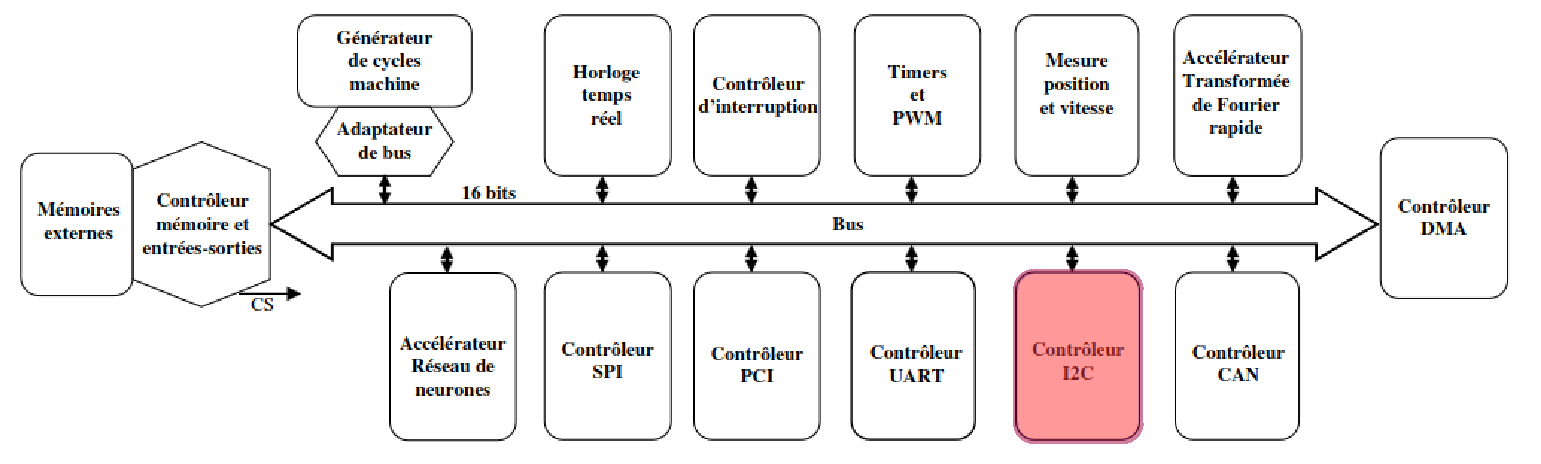
\includegraphics[width=0.95\linewidth]{Images/1_CDC/Architecture.pdf}
    \caption{Architecture du système sur puce considéré}
\end{figure}

Le schéma de câblage du circuit à concevoir est le suivant :
\\

\begin{figure}[H]
    \centering
    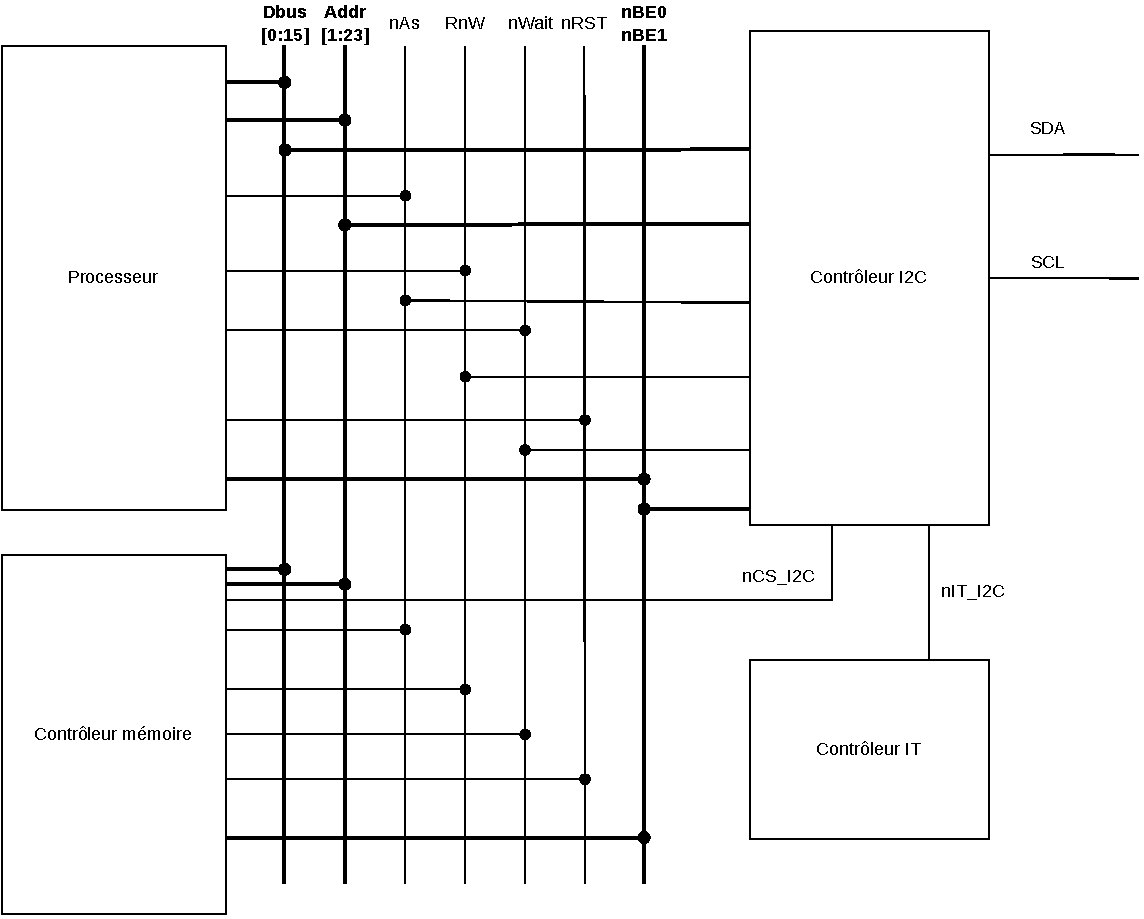
\includegraphics[width=0.95\linewidth]{Images/1_CDC/Schema_cablage.pdf}
    \caption{Schéma de câblage du circuit I2C}
\end{figure}

Les signaux logiques d'entrée-sortie du composant sont résumés dans le tableau suivant
(sens indiqué du point de vue du contrôleur I2C).
\\

\begin{table}[H]
    \centering
    \begin{tabularx}{\textwidth}{|c|c|X|}
        \hline
        \textbf{Nom du signal} & \textbf{Sens} & \textbf{Description} \\
        \hline
        DBus & bidirectionnel & Données codées sur 16 bits, bus de données du processeur \\
        \hline
        Addr & entrée & Données codées sur 22 bits, bus d'adresse du processeur \\
        \hline
        nAS & entrée & Address Strobe, valide la présence d'une adresse sur le bus \\
        \hline
        RnW & entrée & Read not Write, sélection lecture ou écriture \\
        \hline
        nWAIT & entrée & Insertion de cycles d'attente (non utilisé dans le cas du contrôleur I2C : tous les transferts se font en 1 cycle) \\
        \hline
        nRST & entrée & not Reset, signal d'initialisation du circuit \\
        \hline
        CLK & entrée & Clock, horloge du circuit \\
        \hline
        nBE0--nBE1 & entrée & Byte Enable, ordre des octets sur le bus de données \\
        \hline
        nCS\_I2C & entrée & Chip Select, sélection du contrôleur I2C (produit par le contrôleur mémoire et E/S) \\
        \hline
        nIT\_I2C & sortie & Interrupt, signal d'interruption vers le processeur \\
        \hline
        SCL & sortie & Horloge de la liaison I2C \\
        \hline
        SDA & bidirectionnel & Données de la liaison I2C \\
        \hline
    \end{tabularx}
    \caption{Signaux logiques d'entrée-sortie du contrôleur I2C}
\end{table}

\subsection{Chronogrammes caractéristiques}

Cycles d'échange avec le processeur. Les cycles de lecture et d'écriture sont ceux du
bus : synchrone sur CLK, transfert en 1 cycle,
nAS et nBE0-nBE1 actifs pendant le cycle, RnW à 1 pour une lecture et à 0 pour une
écriture. Les écritures concernent la configuration, l'adresse esclave et les données à
émettre ; les lectures concernent le statut et les données reçues.
\\

\begin{figure}[H]
    \centering
    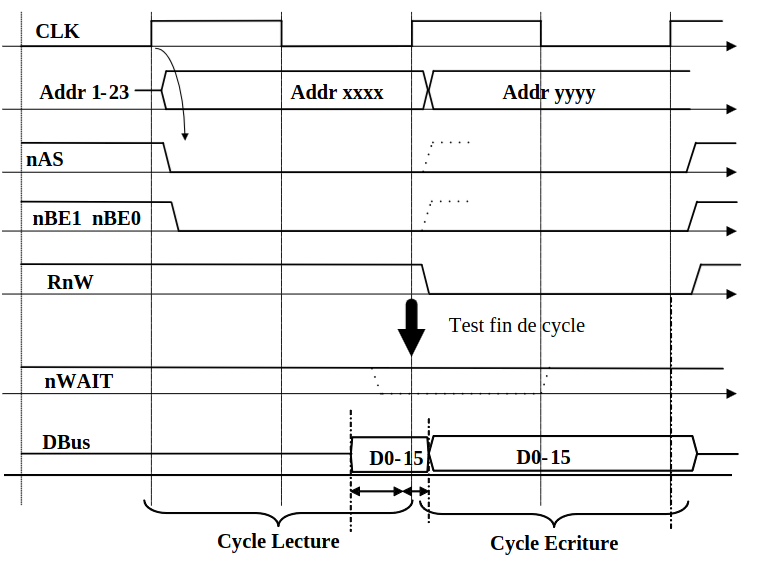
\includegraphics[width=0.95\linewidth]{Images/1_CDC/Cycle_cours.png}
    \caption{Chronogramme des cycles d'échange}
\end{figure}

Les cycles d'écriture permettent soit de configurer les registres du contrôleur I2C, soit d'envoyer des données à transmettre sur la ligne série.
\\

Les cycles de lecture servent soit à consulter les registres d'état du contrôleur, soit à récupérer les données reçues via la liaison série.
\\

La figure suivante illustre le format des trames de données émises et reçues sur le bus série.
\\

\begin{figure}[H]
    \centering
    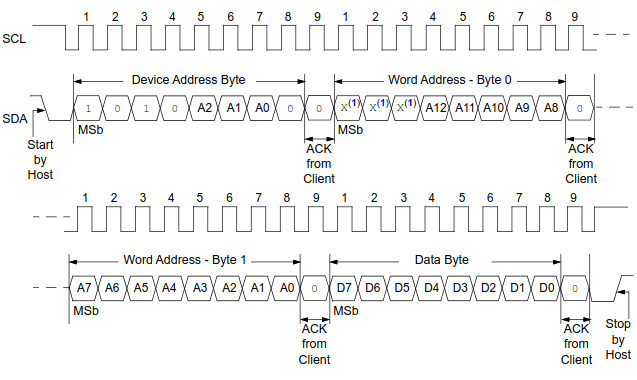
\includegraphics[width=0.95\linewidth]{Images/1_CDC/Trame_I2C_W.png}
    \caption{Chronogramme des trames I2C - Ecriture}
\end{figure}

\begin{figure}[H]
    \centering
    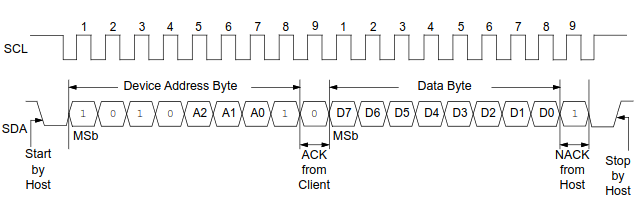
\includegraphics[width=0.95\linewidth]{Images/1_CDC/Trame_I2C_R.png}
    \caption{Chronogramme des trames I2C - Lecture}
\end{figure}

\subsection{Contraintes}

Les contraintes considérées sont celles du projet. Le composant est développé en VHDL
dans l'environnement HDL Designer de Mentor Graphics (saisie, simulation sous
ModelSim, synthèse). Le circuit doit pouvoir être connecté sur le bus imposé, sans
modification de ce dernier, et être réutilisable comme IP.
\\